\section{Our Implementation}

In this section, we describe our implementation of the MoDiff method and the optimizations we obtained.
\subsection{Implementation Details}

We used PyTorch as the deep learning framework for our implementation. The code is based on the official implementation of the MoDiff method, which is available on GitHub. We made some modifications to the original code to adapt it to our specific use case.

To enhance performance, we incorporated the following optimizations:
\begin{itemize}
    \item {\textbf{CUTLASS}} Added CUTLASS(CUDA Templates for Linear Algebra Subroutines and Solvers) to optimize the performance of int8 and int4 convolutions.

    \item {\textbf{Fused Kernels}} Implemented fused kernels for int8 and int4 quantization, dequantization, and activation functions. These fused kernels reduce the overhead of separate quantization and dequantization steps, improving the overall efficiency of the model.

    \item {\textbf{Other Optimizations}} We also implemented consistent buffer management and a channel-last memory format to further optimize performance.
\end{itemize}

\subsection{Benchmarking and Performance}

In order to evaluate the performance of our implementation, we conducted benchmarking experiments. We ran the experiments on a machine equipped with an NVIDIA A40 GPU, using the hyperparameters listed in Table \ref{tab:bench_hyp_table}.

% \begin{table*}
%     [htbp]
%     \centering
%     \begin{minipage}[c]{0.58\linewidth}
%         \centering
%         \begin{tabular}{c|c|c|c}
%             Environment & Value               & Hyperparameter    & Value       \\
%             \hline
%             GPU         & NVIDIA A40          & Model             & LDM         \\
%             OS          & Ubuntu 22.04 Server & Dataset           & LSUN-Church \\
%             PyTorch     & 2.4.0               & Batch Size        & 32          \\
%             Python      & 3.11                & Timesteps         & 200         \\
%             CUDA        & 12.4.1              & Number of Samples & 128         \\
%         \end{tabular}
%         \caption{Benchmark Results for Model Performance Optimization}
%         \label{tab:hyper_table}
%     \end{minipage}
%     \hfill
%     \begin{minipage}[c]{0.38\linewidth}
%         \centering
%         \begin{tabular}{lccc}
%             \toprule \textbf{Mode} & \textbf{FID Score} & \textbf{Samples} \\
%             \midrule FP32          & 5.73               & 50000            \\
%             INT8                   & 5.85               & 50000            \\
%             INT4                   & 14.80              & 50000            \\
%             \bottomrule
%         \end{tabular}
%         \caption{FID Evaluation Results}
%         \label{tab:fid_eval}
%     \end{minipage}
% \end{table*}
\begin{table}
\begin{tabular}{lccc}
    \toprule \textbf{Mode} & \textbf{FID Score} & \textbf{Samples} \\
    \midrule FP32          & 5.73               & 50000            \\
    INT8                   & 5.85               & 50000            \\
    INT4                   & 14.80              & 50000            \\
    \bottomrule
\end{tabular}
\caption{FID Evaluation Results}
\label{tab:fid_eval}
\end{table}

We compared the performance of our implementation with the FP32 generation, the int8-quantized generation without MoDiff, and the int4-quantized generation without MoDiff. The result of our benchmarking is shown in Table \ref{tab:pipeline_speedup} and visualized in Figure \ref{fig:plot_01_pipeline_speedup}.

\begin{table*}
    [bht]
    \centering
    \caption{Running time and DRAM transfer comparison on LSUN-Churches. DRAM transfers include weight, activation, output, cache read, and cache write. Speedup and DRAM transfer reduction are calculated against FP32.}
    \label{tab:pipeline_speedup} \resizebox{\linewidth}{!}{
    \begin{tabular}{lcc|crrrrrrl}
        \toprule & \multicolumn{2}{c|}{Runtime} & \multicolumn{7}{c}{DRAM Transfer (GB)} \\
        \cmidrule(lr){2-3}\cmidrule(lr){4-10} Mode & ms/Sample &  Speedup & Weight & Act & Output & Cache Rd & Cache Wr & Total & Ratio \\
        \midrule FP32 & 613.4 &  1.000$\times$ & 219.2 & 26.3 & 19.2 & 0.0 & 0.0& 264.6 & 100\% \\
        Baseline INT8 & 333.0  & 1.842$\times$& 66.2& 26.3 & 19.2 & 0.0 & 0.0 & 111.6 & 42.2\%  \\
        \textbf{MoDiff INT8 (Ours)}& \textbf{367.7} & \textbf{1.668$\times$} & 66.2& 26.3& 19.2& 51.6  & 36.9& \textbf{200.2} & \textbf{75.6\%}  \\
        Baseline INT4 & 306.2 & 2.003$\times$  & 42.6 & 26.3 & 19.2  & 0.0 & 0.0  & 88.0  & 33.2\%  \\
        \textbf{MoDiff INT4 (Ours)}& \textbf{340.9}& \textbf{1.800$\times$} & 42.6& 26.3& 19.2& 51.6& 36.9& \textbf{176.6} & \textbf{66.7\%}  \\
        \bottomrule
    \end{tabular}}
\end{table*}
\begin{figure*}[ht!]
    \centering
    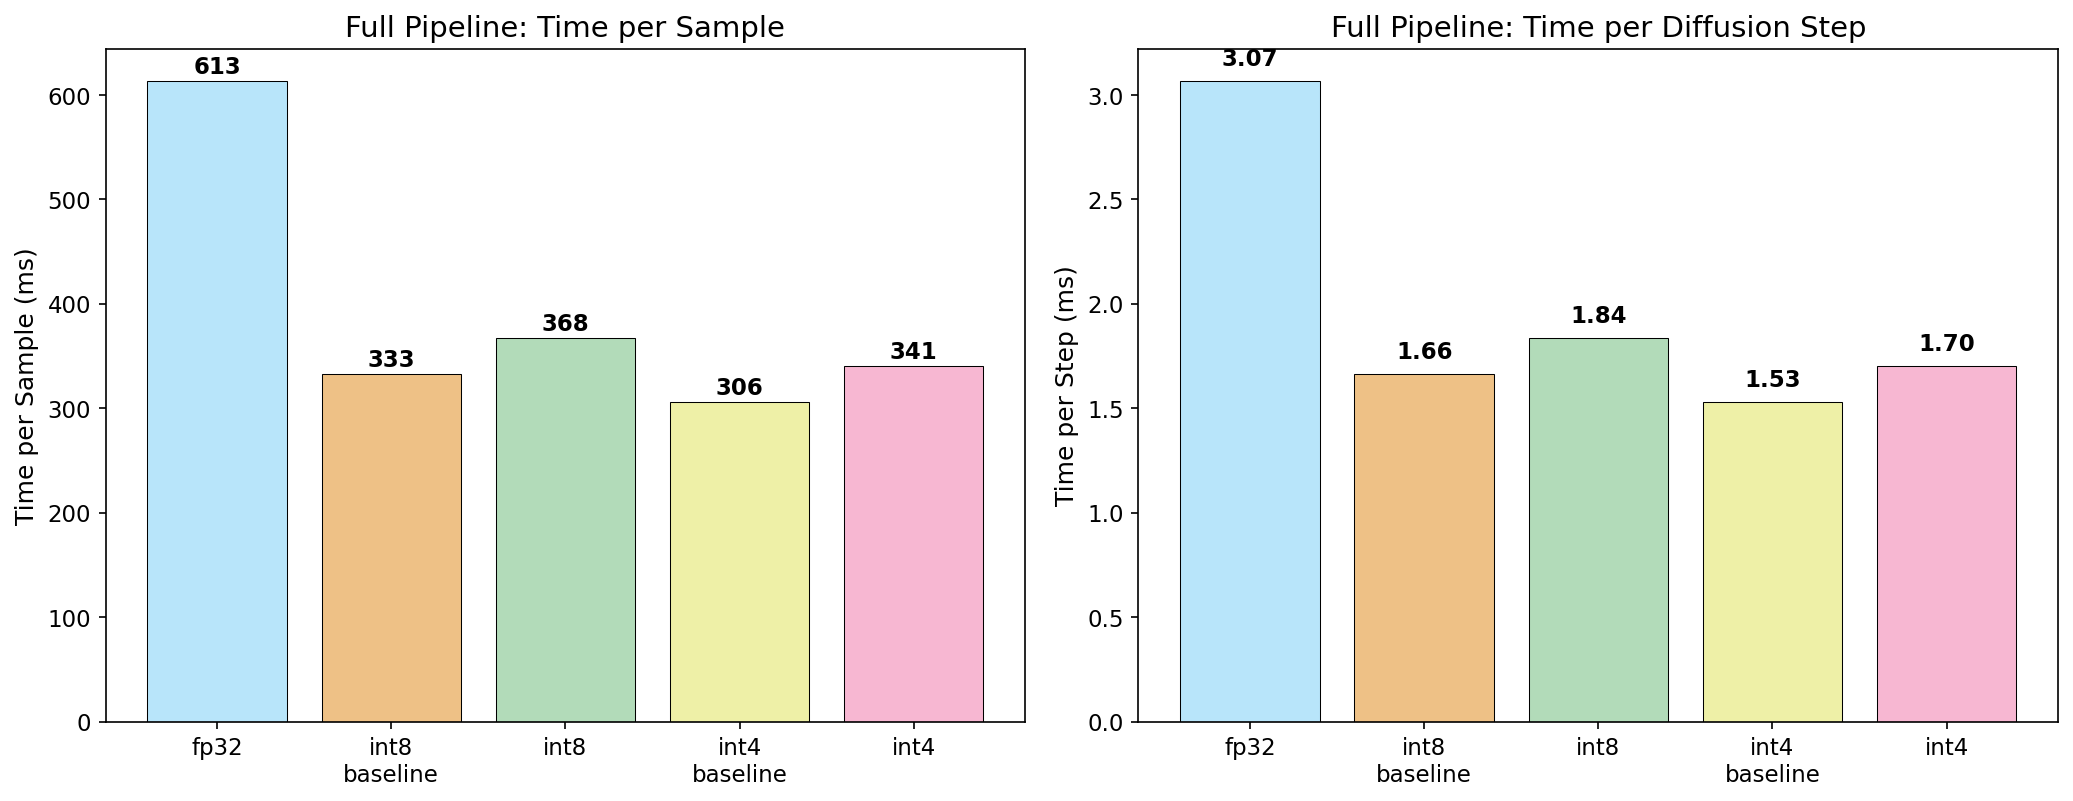
\includegraphics[width=0.8\textwidth]{figures/plot_01_pipeline_speedup.png}
    \caption{Benchmark Results for Model Performance Optimization}
    \label{fig:plot_01_pipeline_speedup}
\end{figure*}

As shown in the results, our implementation of MoDiff with int8 quantization and int4 quantization achieved significant speedups compared to the FP32 generation. The int8-quantized generation with MoDiff achieved a speedup of 1.668x, while the int4-quantized generation with MoDiff achieved a speedup of 1.800x compared to the FP32 generation. These results demonstrate the effectiveness of our optimizations and the potential of MoDiff for accelerating deep learning models.

In order to demonstrate that our implementation meets the quality expectations as the original MoDiff, we also evaluated the quality of the generated images using FID (Fréchet Inception Distance). The FID scores for the FP32 generation, int8-quantized generation with MoDiff, and int4-quantized generation with MoDiff are shown in Table \ref{tab:fid_eval}.

\begin{table}[h]
\centering
\caption{FID Evaluation Results: Quantization vs. FP32 Baseline}
\label{tab:fid_eval}
\begin{tabular}{lccc}
\toprule
\textbf{Mode} & \textbf{FID Score}  & \textbf{Samples} \\
\midrule
FP32 & 5.73 & 50000 \\
INT8 & 5.85  & 50000 \\
INT4 & 14.80 & 50000 \\
\bottomrule
\end{tabular}
\end{table}